
\documentclass[a4paper,12pt,oneside,pdflatex,italian,final,twocolumn]{article}



\usepackage[utf8]{inputenc}
\usepackage{parallel}
\usepackage{siunitx}
\usepackage{booktabs}
\usepackage{fancyhdr}
\usepackage{subfig}
\usepackage[export]{adjustbox}
\usepackage[margin=0.8in]{geometry}
\addtolength{\topmargin}{0in}

\usepackage{libertine}
\renewcommand*\familydefault{\sfdefault}  %% Only if the base font of the document is to be sans serif
\usepackage[T1]{fontenc}
\usepackage{siunitx}
\sisetup{output-decimal-marker={,}}


\title{FICUS software manual for the SESAME-XAFS Detector System}
\author{ReDSoX Collaboration}
\date{October 2019}

\begin{document}

\pagestyle{fancy}

\lhead{ReDSoX Collaboration}
\chead {\today}
\rhead{FICUS Software manual}


\onecolumn

\begin{figure}
\begin{minipage}{0.37\textwidth}
\centering

\includegraphics[width=1\textwidth,left,]{logo_redsox.png}
\end{minipage}
\hfill
\begin{minipage}{0.57\textwidth}
\raggedleft
\vspace{1cm}
\Huge \textbf{FICUS software manual for the SESAME-XAFS Detector System}
    \vspace{2cm}
\end{minipage}
\end{figure}

    
    \tableofcontents 
    
    \vspace{1cm}


\begin{figure} [h]
\begin{minipage}{0.5\textwidth}
\section{Overview}
        Following the beamline requirements, a custom software developed in LabVIEW for data acquisition and instrument management, FICUS (Fluorescence Instrumentation Control Universal Software), was specifically designed.
        

\end{minipage}
\hfill
\begin{minipage}{0.4\textwidth}
\raggedleft
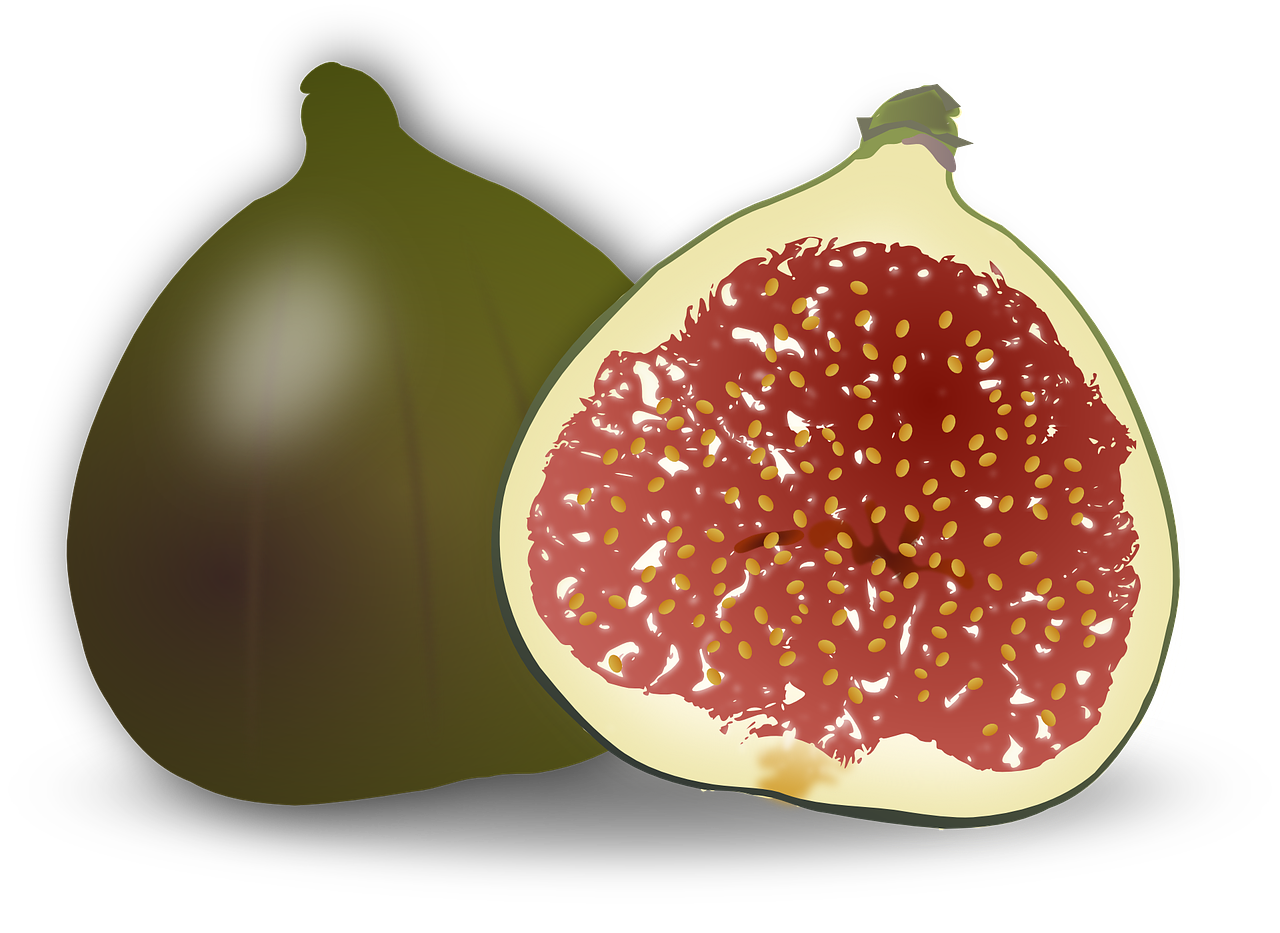
\includegraphics[width=0.6\textwidth,right]{ficus.png}
\caption{FICUS - Fluorescence Instrumentation Control Universal Software}\label{fig:fig0}
\end{minipage}
\end{figure}


        

        

	\clearpage
	
	        \section{Description}
        
       FICUS is a software designed to act on different levels: each level corresponds to a different subject who uses it and, consequently, a different choice of options available. In particular, three levels are available:
       \begin{itemize}
           \item \textbf{Detector Expert}: dedicated to detector and software developers, allows the maximum degree of variation of the available parameters and the display of screens useful for development and debugging;
           \item \textbf{Beamline Staff}: dedicated to the staff of the beamline, allows an intermediate degree of variation of the parameters for the setting and the measurement;
           \item \textbf{User}: dedicated to all possibile users of the beamline, allows a low degree of parameter variation but allows for data collection and pre-analysis.
       \end{itemize}
       
        \section{Applications}
        
        FICUS, after a preliminary selection of measurement parameters, performs the following tasks: data alignment of the cells, energy calibration, selection of the Region Of Interest (ROI). For example, during the measurement it is possible to obtain a spectrum in real time with some information such as FWMH and peak centroid (in ADC channels and in eV), count rate and dead time.
        
        \section{Features}
            \clearpage
	
\section{Guide for Detector Expert}
            %\subsection{Input}

Before starting any activity, please take a look at the \textbf{Safety warnings for using the SESAME-XAFS Detector System}, on page \pageref{accensione}, and the \textbf{Instructions for switching on/off}, respectively on page \pageref{accensione} and \pageref{spegnimento}.

This version of the software is recommended only for developers of the detector system in order to perform extensive testing and optimize performance.

\vspace{1cm}

After the launch of FICUS software, following the instructions recommended in this manual for switching on the detector system, the first window is the one shown in Fig. \ref{fig:fig1}.

        \begin{figure}[h]
        \centering
        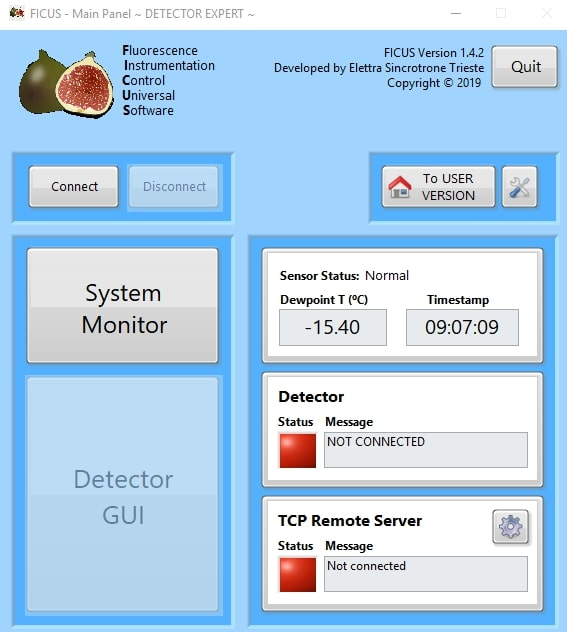
\includegraphics[scale=0.5]{Capture.jpg} \quad %width=0.7\textwidth
        \caption{The first window of FICUS software}\label{fig:fig1}
        \end{figure}
        

\begin{figure}[h]
\centering
\subfloat
{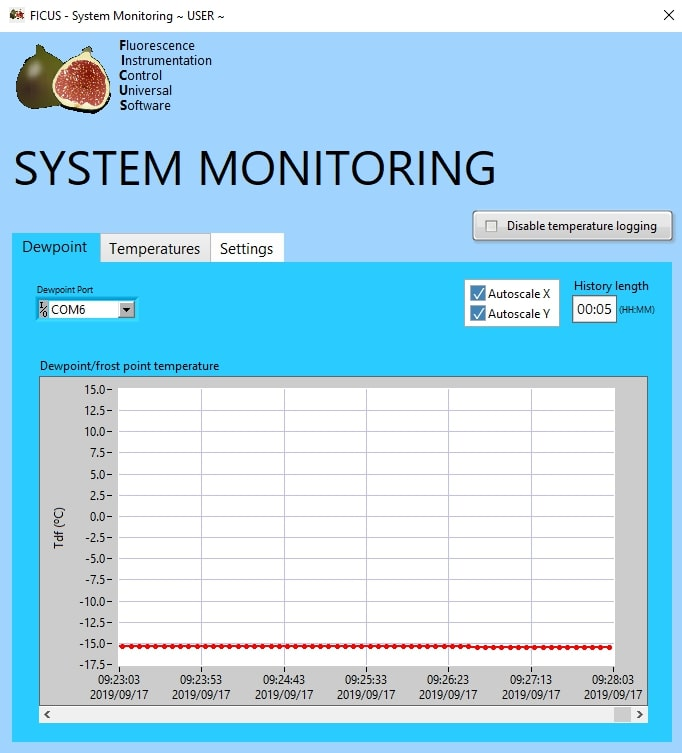
\includegraphics[width=.42\textwidth]{Capture15.jpg}} \quad
\subfloat
{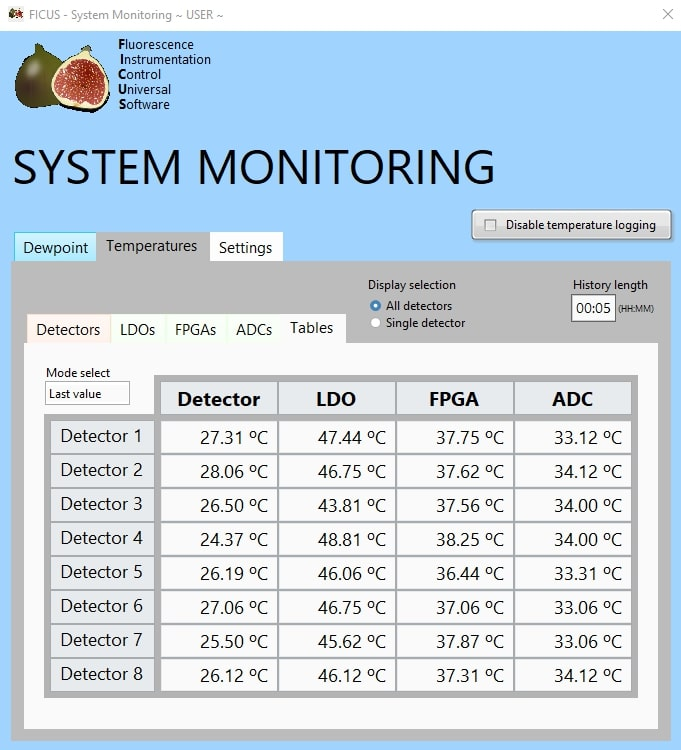
\includegraphics[width=.42\textwidth]{Capture19.jpg}} \\

\caption{(\textbf{a}) The log of the dew point temperature. (\textbf{b}) the table with all the last measured temperatures.}\label{fig:fig2}
\end{figure}

In this window it is possible to see the dew point temperature of the system, the time, the status of the detectors and the status of the TCP Remote Server (red disconnected - green connected). 

After connect of the detector, it is also possible to click on \textit{System monitor} to know: 
\begin{itemize}
    \item the log of the dew point temperature [in Fig. \ref{fig:fig2} (a)]
    \item the log of the temperature of the strips [in Fig. \ref{fig:fig4} (a)]
    \item the log of the temperature of the LDOs [in Fig. \ref{fig:fig4} (b)]
    \item the log of the temperature of the FPGAs [in Fig. \ref{fig:fig4} (c)]
    \item the log of the temperature of the ADCs [in Fig. \ref{fig:fig4} (d)]
    \item the table with all the last measured temperatures [in Fig. \ref{fig:fig2} (b)]
    \item the setting for measuring temperatures [in Fig. \ref{fig:fig3}]
\end{itemize}

In the log it is possible to modify the time duration displayed and to set the extremes of the graph, or to set its auto setting.

\begin{figure}[h]
\centering
{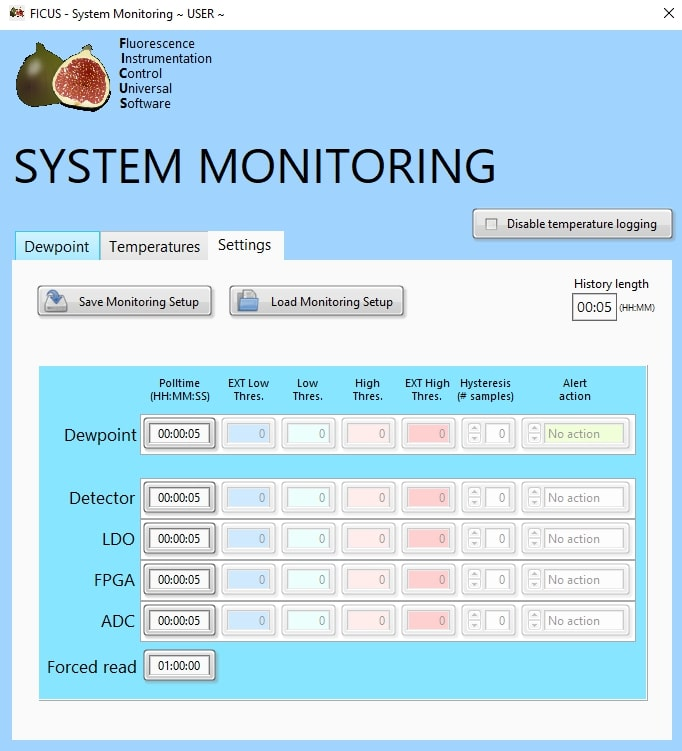
\includegraphics[width=.45\textwidth]{Capture20.jpg}} \quad
\caption{The setting for measuring temperatures.}\label{fig:fig3}
\end{figure}

\begin{figure}[h]
\centering
\subfloat
{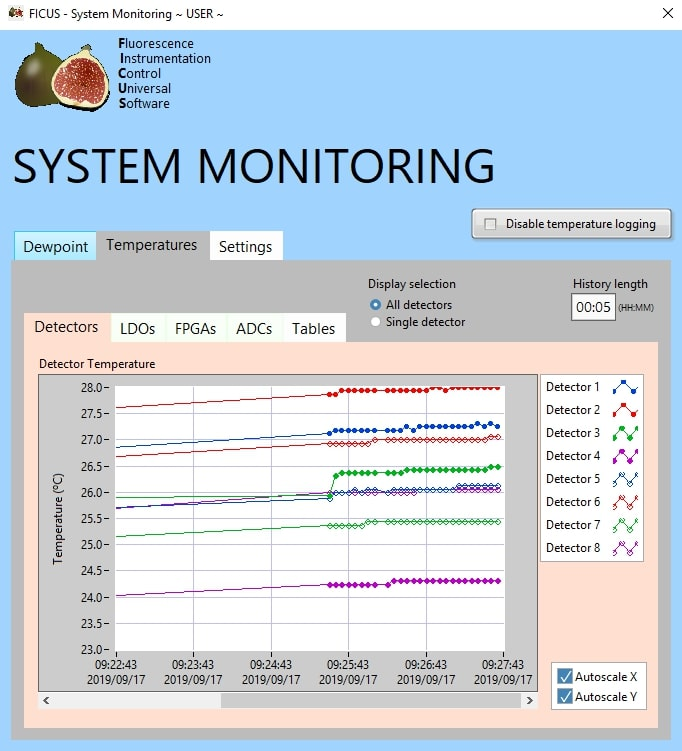
\includegraphics[width=.48\textwidth]{Capture14.jpg}} \quad
\subfloat
{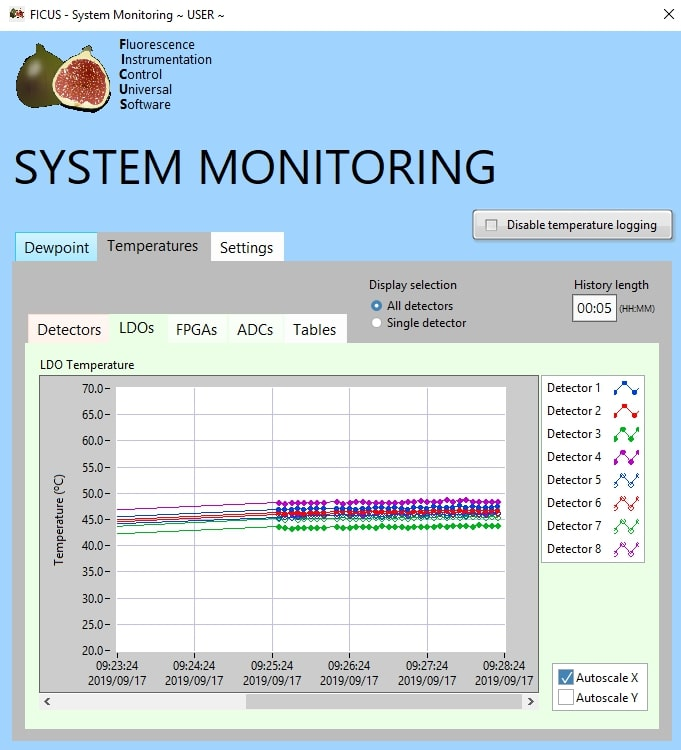
\includegraphics[width=.48\textwidth]{Capture16.jpg}} \\
\subfloat
{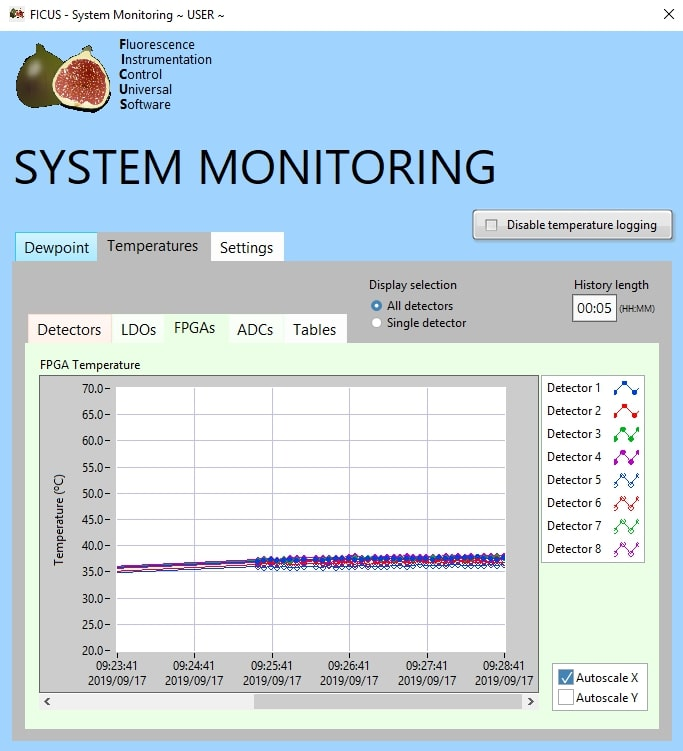
\includegraphics[width=.48\textwidth]{Capture17.jpg}} \quad
\subfloat
{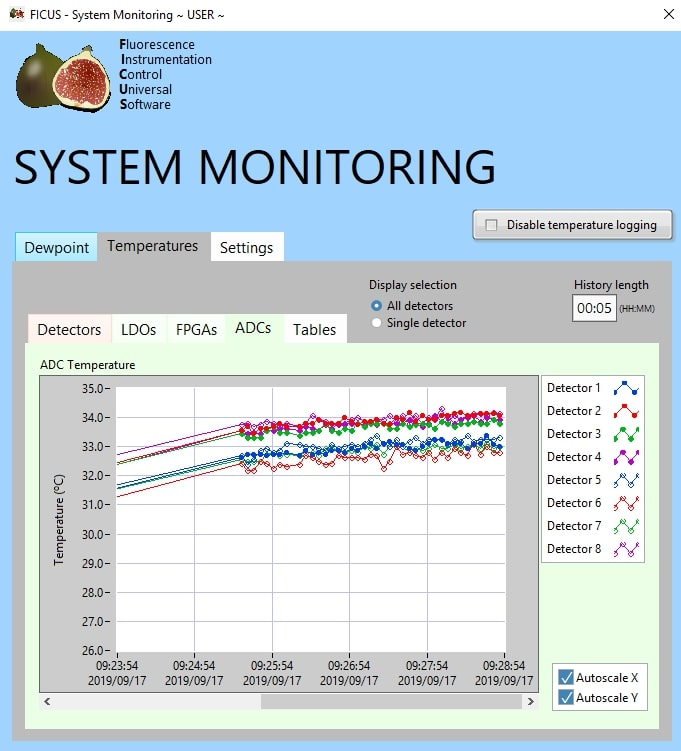
\includegraphics[width=.48\textwidth]{Capture18.jpg}} \\

\caption{In clockwise direction starting from the top left (\textbf{a}) The log of the temperature of the strips. (\textbf{b}) The log of the temperature of the LDOs. (\textbf{c}) The log of the temperature of the FPGAs. (\textbf{d}) the log of the temperature of the ASICs.}\label{fig:fig4}
\end{figure}
\clearpage 

To connect the detector system click on \textit{Connect} (in Fig. \ref{fig:fig1}). The connection window in Fig. \ref{fig:fig5} (a) appears. 
Click on \textit{Run TCP-IP and FPGA tests} and, if the test is successful, all the boxes will be colored green [Fig. \ref{fig:fig5} (b)] and you can proceed to the connection by clicking \textit{OK}.

\begin{figure}[h]
\centering
\subfloat
{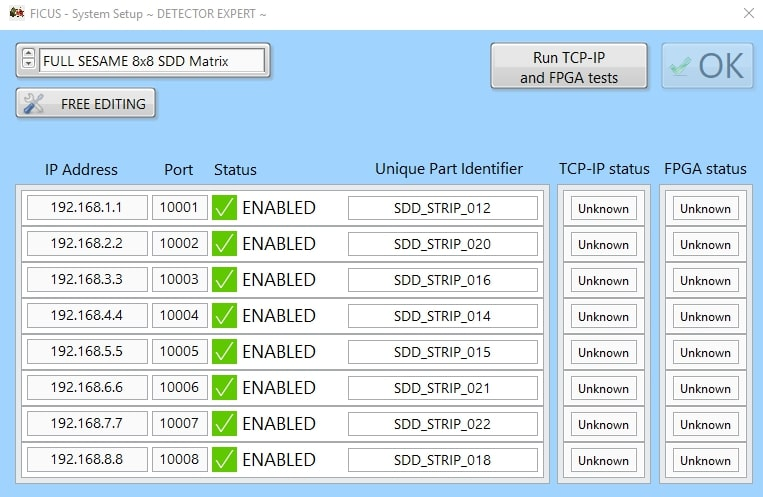
\includegraphics[scale=0.5]{Capture2.jpg}} \\
\subfloat
{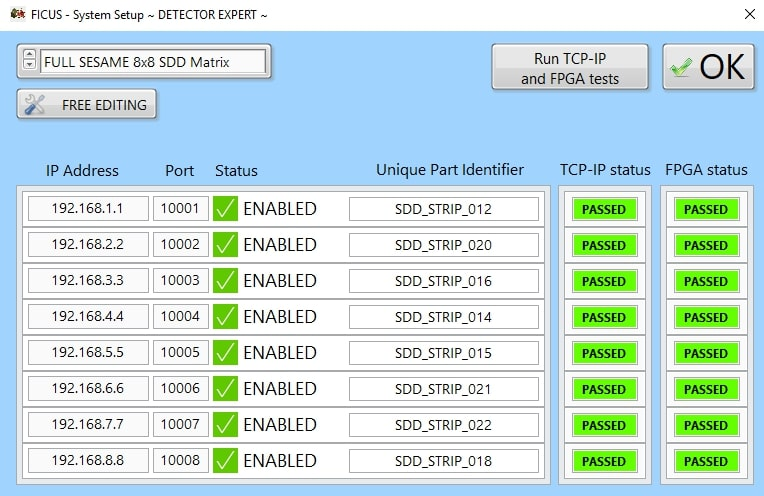
\includegraphics[scale=0.5]{Capture3.jpg}} \\
\caption{(\textbf{a}) The connection window - before connecting tests. (\textbf{b}) The connection window - after passing the connecting tests.}\label{fig:fig5}
\end{figure}

A message appears asking if you want to restore the previously used settings: press \textit{OK} to proceed or \textit{Cancel} to annul the setting restore [Fig. \ref{fig:fig6}]. It is possible to see that the status of the detector has changed to CONNECTED.

\begin{figure}[h]
\centering
{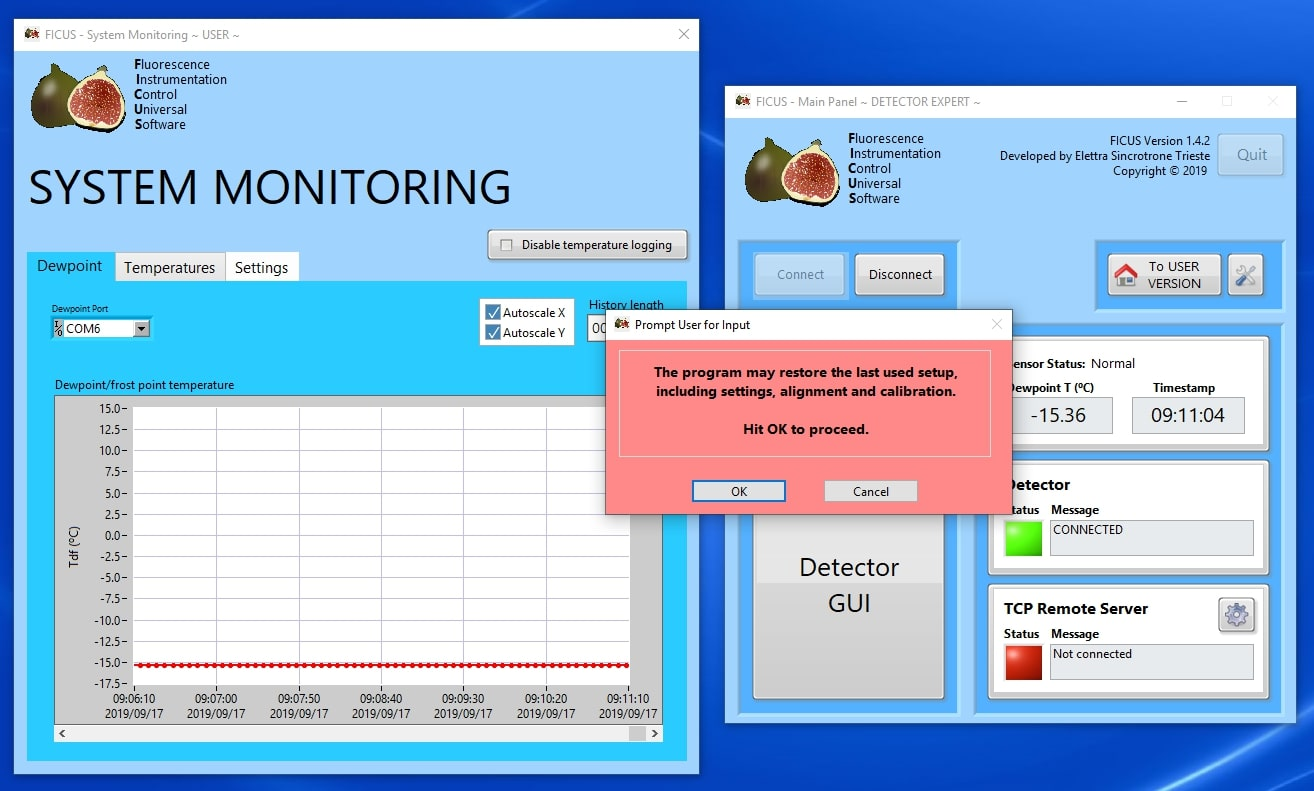
\includegraphics[width=.95\textwidth]{Capture4.jpg}} \quad
\caption{The final window for the connection.}\label{fig:fig6}
\end{figure}

The first windows of the FICUS setting, in Fig. \ref{fig:fig7}, 

\begin{figure}[h]
\centering
{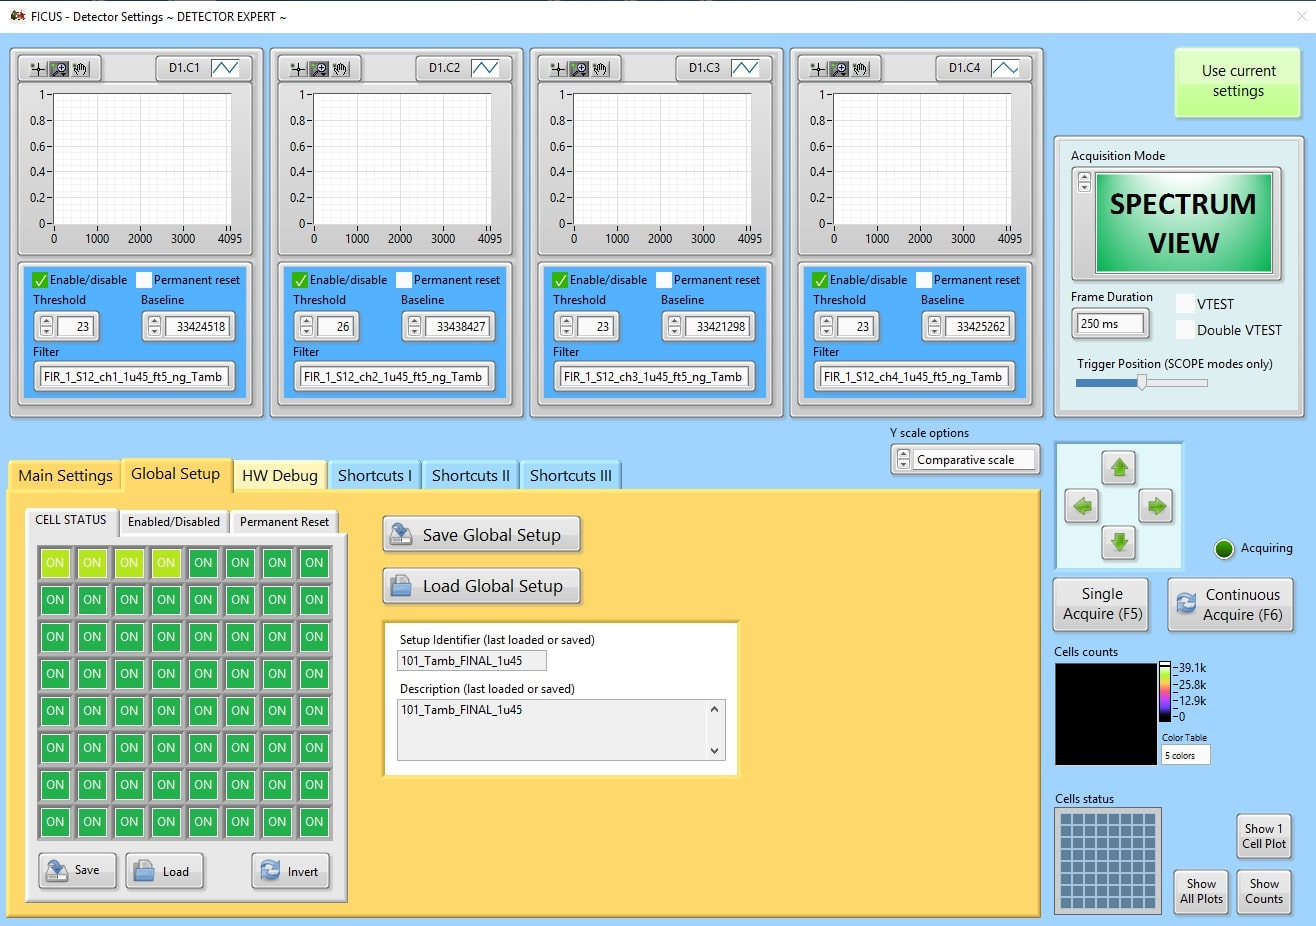
\includegraphics[width=.95\textwidth]{Capture8.jpg}} \quad
\caption{The first windows of the FICUS setting.}\label{fig:fig7}
\end{figure}




























\clearpage

\section{Guide for Beamline Staff}
            %\subsection{Temperature}

Before starting any activity, please take a look at the \textbf{Safety warnings for using the SESAME-XAFS Detector System}, on page \pageref{accensione}, and the \textbf{Instructions for switching on/off}, respectively on page \pageref{accensione} and \pageref{spegnimento}.

This version of the software is recommended for the beamline staff in order to optimize the system settings for the planned measurements.








\section{Guide for User}

Before starting any activity, please take a look at the \textbf{Safety warnings for using the SESAME-XAFS Detector System}, on page \pageref{accensione}, and the \textbf{Instructions for switching on/off}, respectively on page \pageref{accensione} and \pageref{spegnimento}.

This version of the software is useful for the users in order to realize the planned measurements.






%\section{Technical specification}

\section{Safety warnings for using the SESAME-XAFS Detector System} \label{sicurezza}
To use the SESAME-XAFS detector system correctly and avoid damaging the measuring system, you must carefully follow the on/off instructions and the software user's guide.
It's very important:
\begin{itemize}
    \item Never switch the HV power supply off and/or on suddenly: it is important gradually increase or decrease the voltage
    \item Never switch the Peltier cells power supply off and/or on suddenly: it is important gradually increase or decrease the voltage
    \item  If the ambient and system temperatures change, it may be necessary to repeat the procedure for loading the appropriate settings, aligning the cells and calibrating the detector
    \item Make sure that the holes for the nitrogen/dry air vent are not obstructed
    \item Make sure that when the flushing is switched on (with appropriate flow rate) the window just swells up
\end{itemize}

    \subsection{Instructions for switching on} \label{accensione}
  It is very important to follow the switch-on procedure following the steps in order and precisely.
    
    \begin{itemize}
        \item Turn on the PC
        \item Start flushing nitrogen / dry air [maximum flow rate of 2 liter/minute]
        \item Turn on the power supply of the dew point temperature sensor [ch3 - analog power supply]
        \item Launch FICUS software
        \item Check that the dew point temperature is below \SI{16}{\celsius} 
            \begin{itemize}
                \item Only if it is so, activate temperature stabilization and turn on the chiller set to \SI{18}{\celsius} 
                \item If it is not so, wait for the dew point temperature to drop below this value thanks to the flushing
            \end{itemize}
        \item Switch on the digital power supply [all ch1, ch2, ch3, ch4 together]
        \item Switch on the analog power supply [ch1 and ch2 of analog power supply]
        \item From FICUS software connect the detector system
        \item From FICUS software load the appropriate settings according to the condition and temperature of use (possible choice of 8 global setups)
        \item Switch on the HV power supply (setting recall mode1), gradually increase the voltage from 0 V to 60 V on ch1 and then from 0 V to 60 V on ch2
        \item Wait about 5 minutes for the temperature of the detector to stabilize
        \item Proceed with cell alignment (o load a previously saved alignment setting)
        \item Now it is possible activate measurement
        \item After stop the measurement, proceed with the calibration of the detector system (o load a previously saved calibration)
        \item If you want work in cooling mode (to lower cell temperature), start the instruction for cooling mode
        \end{itemize}

	
    \subsection{Instructions for switching off} \label{spegnimento}
      It is very important to follow the switch-off procedure following the steps in order and precisely.
    
    \begin{itemize}
        \item Gradually decrease the voltage from 60 V to 0 V on ch2 and then from 60 V to 0 V on ch1, and after switch off the HV power supply 
        \item In FICUS close the acquisition window and disconnect the detector
        \item Switch off analog power [ch1 and ch2 analog power]
        \item Switch off the digital power supply [all ch1, ch2, ch3, ch4 together]
        \item Turn off FICUS software
        \item Turn off flushing nitrogen / dry air 
        \item For long detector shutdown or if it is necessary, switch off the dew point temperature meter power supply [ch3 - analog power supply] and turn off the chiller
        \item Turn off the PC
    \end{itemize}
    
    \subsection{Instructions for cooling mode} 
     \begin{itemize}
        \item Before starting the Peltier cell ignition procedure, check that the dew point temperature is below \SI{-12}{\celsius}
        \item Never switch the Peltier cells power supply off and/or on suddenly: it is important gradually increase or decrease the voltage
        \item Switching on and off of the Peltier cells have to be gradual: power supply for 0.1 V steps every 2 min (maximum voltage 2 V)
        \item When the supply voltage of Peltier cells is 2 V, wait at least 5 minutes for the temperature of the detector to stabilize
        \item When the cooling mode is activated, remember to load the appropriate global settings [Tcool] in FICUS
    \end{itemize}   
    
\section{Troubleshooting}
In this section a detailing possible errors or problems that may occur, along with how to fix them.

\begin{itemize}
    \item 
    \item 
    \item 
    \item 
    \item 
    \item 
    \item 
    \item 
\end{itemize}

\section{Information \& Contact - ReDSoX Collaboration}
        The FICUS software was developed by Elettra Sincrotrone Trieste.
        
        This software manual has been prepared by the testers of the detector system (detector expert) of INFN-Ts.
        
        The SESAME-XAFS detector system implementation is managed by the Istituto Nazionale di Fisica Nucleare (INFN) in collaboration with Elettra Sincrotrone Trieste, within the ReDSoX (Research Drift detectors for Soft X-ray) collaboration by INFN and Elettra (and other entities listed below in alphabetical order) thanks to ad hoc financing from the Ministry of Education, University and Research (MIUR).
	
        In particular, this work has been made within the ReDSoX-2 INFN research project, supported with the contribution of the Italian Ministry of Education, University and Research within the EUROFEL Project and FBK-INFN agreement 2015-03-06.
	


\end{document}



